\documentclass{exam}
\usepackage{tikz}
\usepackage{circuitikz}
\usepackage{subcaption}

\pagestyle{headandfoot}
\firstpageheader{Name:\underline{\hspace{100pt}}}{}{Date:\underline{\hspace{100pt}}}
\runningheader{}{\textbf{Kinematics}}{}
\firstpagefooter{The Aetherius Olympiad in Physics}{\thepage}{}
\runningfooter{The Aetherius Olympiad in Physics}{\thepage}{}

\begin{document}

\begin{center}
    \LARGE{\textbf{The Aetherius Olympiad in Physics}}

    \vspace{8pt}

    \large{2023-10}
\end{center}

\section*{Instructions}
\begin{itemize}
    \item You must immediately fill out your name as well as the current date on the top of the page.
    \item You will be given 30 minutes to complete 3 questions. No extra time is allowed, and one must stop writing as soon as the time is up.
    \item You will have to show adequate work to prove that your answer was the result of thoughts but not guesses or anything else.
    \item You must explicitly indicate what your final answer is (\textit{e.g.} circling, boxing, etc).
    \item All questions would be scored out of 5, and one would receive scores based on not only the right answer, but also on the attempt, logic, and thought. A mere correct answer may not necessarily earn full marks.
    \item Scratch paper would be provided upon request. One may not use their own scratch paper.
    \item You may begin as soon as the timer starts.
\end{itemize}

\section*{Questions}

\begin{questions}
    \question[5]{Suppose an object $ O $ is launched at some angle relative to the horizontal and its initial height is equal to its final height. Assume that the gravitational acceleration is constant, at what angle should $ O $ be launched to achieve the greatest range?}

    \pagebreak

    \question[5]{
        A capacitor is a device which can store electrical charge. Current can flow freely through a capacitor when its uncharged just like it does on wires, but if the capacitor is charged, current cannot flow through it. Assume an ideal condition where no charges leak from an isolated capacitor after it's charged. Given the two circuits above, after the batteries are disconnected, in which case would the capacitor retain its charge after a long period of time?

        \begin{figure}
            \begin{subfigure}{0.5\textwidth}
                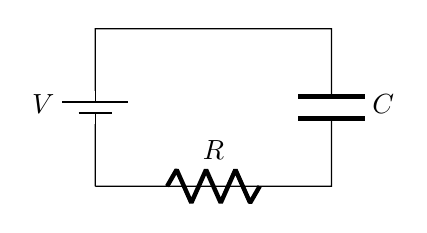
\begin{tikzpicture}
                    \tikzstyle{mybattery}=[battery1,l=$V$,invert]
                    \tikzstyle{thick C}=[C,thick,l=$C$]
                    \draw (0,0) to[mybattery] (0,2) -- (3,2)
                    to[thick C] (3,0) -- (0,0)
                    to[R, l=$R$] (3,0) -- (3,0)
                    ;
                    \node at (-0.35,0.7) {};
                    \node at (-0.35,1.4) {};
                    \node at (3.3,0.65) {};
                    \node at (3.3,1.45) {};
                \end{tikzpicture}
            \end{subfigure}%
            \begin{subfigure}{0.5\textwidth}
                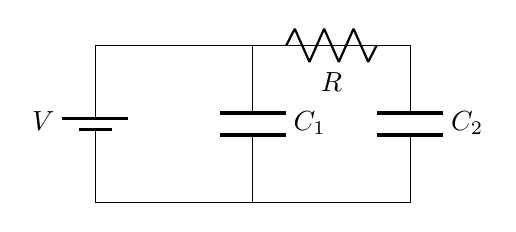
\begin{tikzpicture}
                    \tikzstyle{mybattery}=[battery1,l=$V$,invert]
                    \tikzstyle{thick C}=[C,thick,l=$C$]
                    \draw (0,2) to[short] (2,2) to[thick C,l=$C_1$] (2,0) to[short] (0,0);
                    \draw (2,2) -- (4,2) to[R, l=$R$] (2,2) -- (4,2) to[thick C,l=$C_2$] (4,0) -- (2,0);
                    \draw (0,0) to[mybattery] (0,2) -- (3,2);
                \end{tikzpicture}
            \end{subfigure}
        \end{figure}
    }

    \pagebreak

    \question[5]{Given the following configuration in space, assume that at infinity, electric field is zero. What is the potential energy of the system?
        \begin{center}
            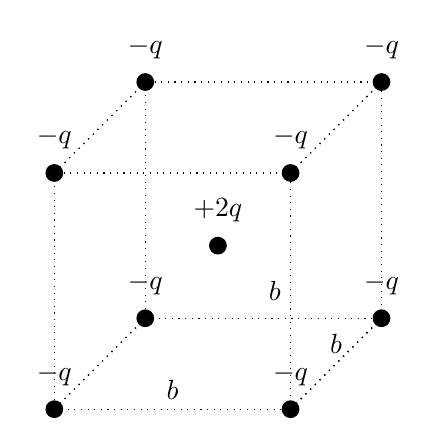
\begin{tikzpicture}[scale=3]
                \coordinate (A) at (0,0,0);
                \coordinate (B) at (1,0,0);
                \coordinate (C) at (1,1,0);
                \coordinate (D) at (0,1,0);
                \coordinate (E) at (0,0,1);
                \coordinate (F) at (1,0,1);
                \coordinate (G) at (1,1,1);
                \coordinate (H) at (0,1,1);
                \coordinate (M) at (0.5,0.5,0.5);

                \foreach \point/\label in {A/-q, B/-q, C/-q, D/-q, E/-q, F/-q, G/-q, H/-q, M/+2q}
                \filldraw (\point) circle (1pt) node[above=5pt] {$\label$};

                \foreach \pointA/\pointB/\label in {A/B/, B/C/, C/D/, D/A/, E/F/b, F/G/b, G/H/, H/E/, A/E/, B/F/b, C/G/, D/H/, A/E/, B/F/, C/G/, D/H/}
                \draw[dotted] (\pointA) -- (\pointB);
                \draw[dotted] (E) -- (F) node[midway, above] {$ b $};
                \draw[dotted] (B) -- (F) node[midway, above] {$ b $};
                \draw[dotted] (F) -- (G) node[midway, left] {$ b $};
            \end{tikzpicture}
        \end{center}
        Hint: The potential energy between two particles is given as $ E_{p} = k \frac{q_1q_2}{r}$.
    }
\end{questions}

\end{document}